\chapter{Soni trapeze}\label{chapter:Soni_trapeze}

\section{Purpose}

This test case aims at validating the closure {\em uniform erosion -- uniform deposition}
imposed on the evolution of cross-section in deposition context, see the Courlis' user document.
For this purpose, we have reused the same configuration than the Soni test case
and just replaced the geometry of rectangular channel by a trapezoidal one.

\section{Description}

We refer to Chapt. \ref{chapter:Newton_trapeze} for the equations on construction of
a trapezoidal cross-section from a given rectangular one. Now, applying these equations
for the Soni test case for which $\epsilon = 0.35$ and by fixing $\alpha = 0.4$,
one can find $\beta = 0.2368$ and $B/L = 1.5088$. The resulting trapezoidal cross-section
is sketched in Fig. \ref{soni_trapeze:fig:profile_init}.

\begin{figure}[!ht]
 \centering
 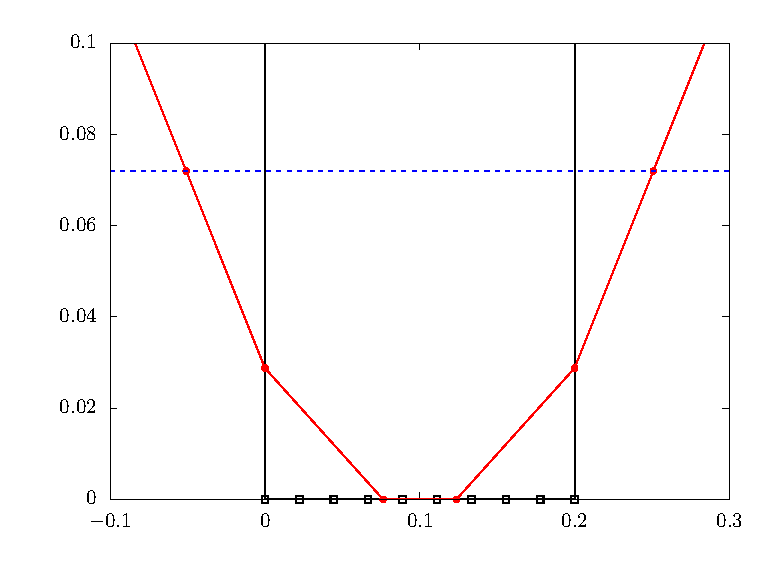
\includegraphics[width=0.9\textwidth]{profile_init.pdf}
 \caption{Initial cross-section.}
 \label{soni_trapeze:fig:profile_init}
\end{figure}

Next, for the chosen closure {\em uniform erosion -- uniform deposition}, we have
imposed the width of erosion parameter being the larger base $P_2P_5 = L$. Recall
that according to this closure, the trapezoid $P_2P_3P_4P_5$ will be moved upward
with some distance $\delta z$ in case of deposition.

\section{Results}

Figure \ref{soni_trapeze:fig:sarap} shows the results with the Sarap kernel.
Figure \ref{soni_trapeze:fig:rezo} shows the results with the Rezo kernel.
One can note that the feature is not yet avaliable with the Mascaret kernel.
In particular,
the number of call on the planimetrage routine is shown in the left plots. One can
find that re-planimetrage was only carried out where the river bottom is deposed.
\begin{figure}[!ht]
 \centering
 \includegraphicsmaybe{[width=0.9\textwidth]}{../img/sarap_plong.png}
 \includegraphicsmaybe{[width=0.9\textwidth]}{../img/sarap_ptravers.png}
 \caption{Longitudinal and tranversal profiles given by the Sarap kenel.}
 \label{soni_trapeze:fig:sarap}
\end{figure}

\begin{figure}[!ht]
 \centering
 \includegraphicsmaybe{[width=0.9\textwidth]}{../img/rezodt_plong.png}
 \includegraphicsmaybe{[width=0.9\textwidth]}{../img/rezodt_ptravers.png}
 \caption{Longitudinal and tranversal profiles given by the Rezo kenel.}
 \label{soni_trapeze:fig:rezo}
\end{figure}

\section{Conclusion}
The evolution of cross-sections is correctly reproduced.
